\chapter{System Implementation} \label{chap:sysImplementation}
%\version{v1.10.2015}

\section*{}
The process of turning an idea into a reality is called implementation. Implementation of a technical specification or an algorithm, in the form of a program or a software component or in any other form a computer system, is the process of programming and deployment. In the case of Indus Bazar, the implementation is the translation of the architectural design of a B2B/B2C marketplace into a fully functioning Flutter-based mobile application backed by a cloud computing server that allows manufacturers, wholesalers, and retailers in the entire country of Pakistan to connect, negotiate, and conduct business in one cohesive digital platform.

\section{System Architecture}

Indus Bazar is designed on a strong 3-Tier Architecture which provides a scalable, maintainable and secure B2B marketplace experience. This design ensures there is a well-defined division of responsibilities at the presentation layer (user interface), application layer (business logic), and data layer (database management). The system enables these components to be independently developed, tested and deployed, which greatly increases flexibility and minimizes the complexity of the system.The presentation layer gives manufacturers and buyers a user-friendly and responsive interface to make user experience cross-user activities smooth. Core functionalities like user authentication, product management, order processing and real time communication regulated by business rules and data consistency are dealt with by the application layer. In the meantime, the data layer safely handles all transactional and user information, facilitating effective storage, retrieval and integrity by optimizing the database design.This layered design improves the performance of the system, enables both horizontal and vertical scaling and improves on security since the layers are limited in direct contact.It also makes future upgrades, addition of new functionalities (including AI-based suggestions or analytics), and maintenance simpler and Indus Bazar a brand of modern B2B commerce in the future.
\begin{figure}[H]
\centering
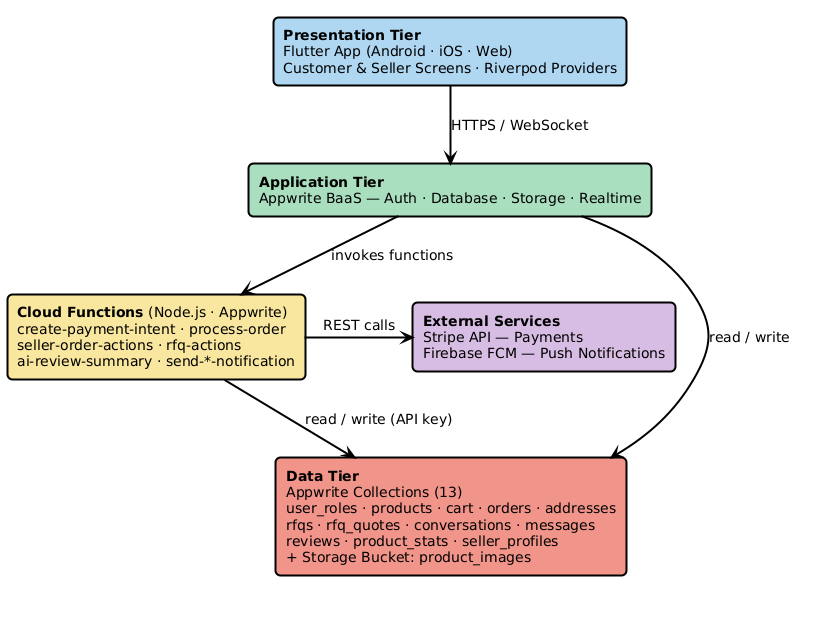
\includegraphics[width=1.0\textwidth]{figures/pictures project/Architecture.png}
\caption{Indus Bazar 3-Tier System Architecture}
\label{fig:system_architecture_implementation}
\end{figure}

The architectural diagram shown in Figure \ref{fig:system_architecture_implementation} depicts the entire 3-level model of the Indus Bazar B2B marketplace. The individual tiers have different functions and they work harmoniously together to provide a cohesive digital commerce platform between manufacturers, wholesalers and retailers in Pakistan.

\subsection{Presentation Tier - User Interface Layer}
Presentation level is the main interaction point between the customers and sellers with the Indus Bazar. This interface is developed with Flutter (Dart), a high-performance, cross-platform mobile application that is natively supported on Android and can be accessed through the web, providing a consistent and user-friendly user experience, no matter the device used.

\subsubsection{Customer Interface Components:}
\begin{itemize}
    \item \textbf{Customer Login Interface:} Customer Login with secure authentications and access to the personalised customer role-based routing with an AppWrapper widget as a dashboard.
    \item \textbf{Product Browse Screen:} Advanced product catalogue category filter, key word search, and treading stacked bulk pricing showcase effective product exploration.
    \item \textbf{Product Detail Screen:} Product in detail with multi-image gallery, full order-based real-time tiered pricing recalculation, specifications and seller information, quantity.
    \item \textbf{Cart and Checkout:} Smoother cart operations with price tier resolving quantity-awareness, address delivery choice, and built-in Stripe payment sheet to secure payments.
   \item \textbf{Order Management:} Full order history and live tracking of status (pending, confirmed, shipped, delivered) with push notification notifications at every lifecycle transition.
   \item \textbf{RFQ Marketplace:} Request for Quotation interface which enables customers to post procurement order, check out competitive seller quotes and take the best offer and move on to payment.
   \item \textbf{Real-Time Chat:} In-built messaging system to communicate directly with the buyer and seller, advertising text and picture messages with live unread badge counters.
  \item \textbf{Intelligent product review interface:} An interface that demonstrates the AI generated summaries of feedback of customers in English and Urdu to be informed in making their purchase decisions.
  \item \textbf{Address Management:} Multi address management screen to enable customers to add or edit their addresses and choose delivery addresses when making the checkout.
\end{itemize}

\subsubsection{Seller Interface Components:}
\begin{itemize}
   \item \textbf{Seller Dashboard:} Headquarters to deal with product listings, track incoming orders, and the reply to proactive RFQ requests in the marketplace.
   \item \textbf{Product Management:} Complete product life cycle management such as add, edit and deactivate multiple image upload and adjustable tiered pricing models.
   \item \textbf{Order Fulfilment:} Status progression controls (confirm, deliver, cancel) and Seller-side order management, and automatic push notifications to the customers at every stage.
   \item \textbf{RFQ Response System:} Open RFQ marketplace view where the sellers can browse the active one, respond to customer requests, provide competitive quotes, and handle orders converted to accepted quotes.
   \item \textbf{Seller Profile:} Business profile management such as business name, city, contact. The information, profile picture, and average customer rating would be shown to all purchasers.
   \item \textbf{Chat Interface:} Live chatting with the customers to explain the specifications of the products, price negotiation, and establish business relationships in the long term, directly on the platform.
    
\end{itemize}

\subsection{Application Tier - Business Logic Layer}
Application Tier involves the business logic of the platform and is where all the operations of the system are coordinated. Developed on a Backend-as-a-Service (BaaS) based on Appwrite and eight Node.js serverless cloud functions, this layer makes sure the communication between the user interface and the underlying data systems is secure and efficient.

\subsubsection{Core Application Modules:}
\begin{itemize}
    \item \textbf{Authentication Service:} Provides secure user registration, enforcement of email verification, session management based on roles, and deep links to password recovery with Appwrite Account APIs and deep link schemes (indusbazar://verify and indusbazar://reset-password).
    \item \textbf{Product Catalogue Engine:} Processes product listings, category searches, search indexes, stock tracking, and tiered price logic, secure bulk price resolution on the basis of order quantity limits set on a product basis.
    \item \textbf{Payment Processing Function (create-payment-intent):} a cloud based on the server-side Node.js function to make Stripe PaymentIntents and Customer objects safely, guaranteeing the Stripe secret key is never sent to the client.
    \item \textbf{Order Processing Function (process-order):} Processes atom order creation, stock de-To avoid overselling under a single server-side transaction, a single server-side transaction is done to induce, and cart clearing concurrent customer orders.
    \item \textbf{RFQ Actions Function (rfq-actions):} The overall RFQ lifecycle includes status transitions (open, quoted, accepted, expired, cancelled), quote submission, quote acceptance.
    \item \textbf{Seller Order Actions:} The Seller Order Actions thing lets sellers list and update the status of orders. They can use an API key to get around the security that's in place for customers. This way sellers can still keep all the data safe.
    \item \textbf{AI Review Summary:} The AI Review Summary thing uses the Google Gemini API to make summaries of what customers are saying. These summaries are in two languages, English and Urdu. The summaries are stored in a place so they can be found quickly.
    \item \textbf{Notification Functions:} There are some functions that send notifications to peoples phones. These functions are called send-order-notification, send-chat-notification and send-rfq-notification. They use Firebase Cloud Messaging to send the notifications in time.
    \item \textbf{Real-Time Chat Engine:} The Real-Time Chat Engine is like a messaging system. It uses Appwrite Realtime WebSocket subscriptions to send messages away. It also updates the count of messages in real time so people can see when they have new messages without having to check all the time.

\end{itemize}

\subsection{Data Tier - Information Storage Layer}
The Data Tier provides secure and efficient data persistence through Appwrite's NoSQL document database and cloud storage, ensuring data consistency, integrity, and availability across all platform operations. This layer manages the complete lifecycle of marketplace data while complying with privacy and security requirements through document-level Row-Level Security (RLS) enforced at the Appwrite platform level.

\subsubsection{Database Components:}
\begin{itemize}
    \item \textbf{user-roles Collection:} This collection contains the mapping between the Appwrite user IDs, which are assigned roles (Customer or Seller), and FCM push notification tokens to deliver targeted notifications.
    \item \textbf{products Collection:} The main product catalogue where the product name, description, classification, inventory levels, status, seller presentations, and levels of price reduction are stored. It supports up to three price levels with minimum quantity limits.
    \item \textbf{cart Collection:} Stores customer cart items connecting user IDs to product IDs with selected quantities, with real-time recalculation of tiers in the checkout flow.
    \item \textbf{orders Collection:} Contains finalized records of orders including customer information and JSON-encoded item arrays (productId, productName, price, quantity, sellerId), amount paid, purchase intent, delivery address, reference address, approximate delivery date, and order lifecycle status.
    \item \textbf{addresses Collection:} Records customer delivery addresses including full name, phone number, street lines, city, province, postal code, and country, along with a default address flag for streamlined checkout.
    \item \textbf{seller-profiles Collection:} Stores seller business profile data such as business name, description, phone, address, city, profile image URL, and a lowercase city field for case-insensitive geographic search.
    \item \textbf{reviews Collection:} The reviews collection contains product review records. These records include a rating from 1 to 5, a title, a comment, image URLs, a flag indicating whether the purchase was verified, a helpful count, and tracking of users who found the review helpful. This ensures the authenticity of reviews.
    \item \textbf{product\_stats Collection:} This collection stores rating statistics for each product. It includes the overall rating, total number of reviews, and the count of reviews for each rating from 1 to 5. This allows efficient display of statistics without real-time computation.
    \item \textbf{conversations Collection:} Stores chat threads. Each thread is identified by the customer ID, seller ID, and product ID. It also includes a preview of the latest message, timestamp, and the number of unread messages for each user.
    \item \textbf{messages Collection:} Stores individual chat messages linked to conversation threads. Each message contains the sender's ID, message text, an image URL, and a timestamp. It also tracks read status and updates for each message.
   \item \textbf{rfqs Collection:} Stores Request for Quotation (RFQ) documents. Each record includes customer ID, product name, category, quantity, delivery city, deadline, specifications, optional target price range, and current status.
   \item \textbf{rfq\_quotes Collection:} Contains quotes submitted by sellers for RFQ documents. It records unit price, lead time in days, notes, and acceptance status.
   \item \textbf{review\_summaries Collection:} Caches AI-generated review summaries. The ai-review-summary cloud function manages these records to reduce API calls to Gemini and improve response times.
   \item \textbf{Appwrite Storage (product\_images):} This storage bucket is used for product catalogue images and review attachment images. MIME types are validated at both the client side and bucket level to ensure file integrity and security.
\end{itemize}
The Indus Bazar platform has a 3-tier architecture that makes it a reliable and intelligent B2B marketplace. This means Indus Bazar is flexible.
Indus Bazar delivers data security, user privacy and commercial performance at a high level.The different parts of the Indus Bazar platform work together to make sure data moves freely.The Indus Bazar platform responds to what each user needs. It does this in real time.This helps Indus Bazar support all the things that need to happen in a B2B marketplace, in Pakistan.

\section{System Internal Components}
There are working parts of Indus Bazar. These sections assist in offering a service between businesses to purchase and sell with one another.Every section has a task to play. This makes the system to work and provides users with an experience.The platform is used by customers and sellers.They receive the potential experience whilst utilizing Indus Bazar.Indus Bazar ensures that it is easily usable by customers and sellers.It assists them to transact business with one another.
\subsection{System Functionality Overview}
The system consists of components that interact with each other. These segments are puzzle segments that will be assembled to give an online shopping system. They collaborate well to provide businesses with a secure and excellent place to market products online. This suits any type of businesses be it the shops or large factories. The system possesses features and is geared towards the people in Pakistan. The system is also secure meaning that it safeguards businesses utilizing it. Pakistani businesses of all sizes can use this system from retailers, to large manufacturers.

\subsubsection{Core Functional Components}

\paragraph{Authentication and User Management System}
Authentication system offers secure access control with industry-standard Appwrite Account APIs. It serves multi-role user registration (Customer and Seller), deep link-based enforcement of email verification, session management and password recovery. The AppWrapper widget constantly checks the authentication and email verification status and does not allow a user to access any dashboard screen until verified. Role assignment gets stored in the collection of user roles as soon as an account is created, and the dashboard can be routed properly, and feature access is granted even during the first login.

\paragraph{Product Catalogue and Search Engine}
This component manages the complete product discovery and management experience, including:
\begin{itemize}
    \item \textbf{Product Listings:} Organized catalogue, categorized, and searchable by keyword to enable effective product discovery within the marketplace.
    \item \textbf{Tiered Bulk Pricing:} Unit price is automatically recalculated according to configured quantity thresholds (volume-based B2B purchases with up to three pricing levels per product), allowing bulk purchasing with transparent pricing.
    \item \textbf{Multi-Image Gallery:} Product images are uploaded to Appwrite Storage and displayed with effective caching to ensure a smooth and fast browsing experience.
    \item \textbf{Seller Product Management:} Sellers can add, edit, and deactivate products with full control over stock quantities, pricing, and product visibility across the platform.
\end{itemize}

\paragraph{Cart and Checkout System}
The cart and checkout module provides a streamlined purchasing workflow from product selection to payment confirmation:
\begin{itemize}
    \item \textbf{Intelligent Cart Management:} Real-time tiered recalculation of prices with changing quantities, ensuring customers always view accurate bulk pricing before checkout.
    \item \textbf{Delivery Address Selection:} Integration with an address management system to allow selection of stored or new delivery addresses during checkout.
    \item \textbf{Stripe Payment Integration:} Secure payment intent creation on the server via cloud operations, with a native Stripe payment sheet for entering credit card details in a PCI-compliant manner, followed by transaction confirmation.
    \item \textbf{Atomic Order Processing:} Cart clearance, stock deduction, and post-payment order creation are handled atomically on the server side through the process-order cloud engine to prevent inventory inconsistencies during parallel orders.
\end{itemize}

\paragraph{Order Management System}
The order management module handles the full commercial lifecycle from order placement to final delivery:
\begin{itemize}
    \item \textbf{Customer Order Tracking:} Real-time monitoring of order status (pending, confirmed, shipped, sent), with push notifications at every status change to keep buyers informed.
    \item \textbf{Seller Order Fulfilment:} Seller dashboard controls for managing order status progression, detailed views of order items, customer delivery address, special notes, and estimated delivery date management.
   \item \textbf{Server-Side RLS Bypass:} Seller order status updates are handled through the seller-order-actions cloud function using an Appwrite API key, enabling secure updates to customer-owned order data without compromising data integrity.
\end{itemize}

\paragraph{RFQ (Request for Quotation) System}
The RFQ module introduces competitive procurement capability that is entirely absent from all existing competing platforms in the Pakistani B2B market:
\begin{itemize}
    \item \textbf{Customer RFQ Submission:} Customers can post procurement requests including product name, category, required quantity, delivery city, submission date, technical specifications, and an optional target price range.
    \item \textbf{Open RFQ Marketplace:} RFQs are publicly visible to all registered sellers, enabling simultaneous competitive bidding and effective price discovery across the platform.
    \item \textbf{Quote Submission and Acceptance:} Sellers submit quotes with unit price, total price, lead time (in days), and additional notes. Customers review all received quotes and select the most suitable offer.
    \item \textbf{RFQ-to-Order Conversion:} Accepted quotes are automatically converted into a standard Stripe payment and checkout process, where a confirmed order is generated upon successful payment processing.
    \item \textbf{Push Notification Integration:} When a new RFQ is created, immediate notifications are sent to all registered sellers via the send-rfq-notification cloud service to maximize response rates and competition.
\end{itemize}

\paragraph{Real-Time Chat and Messaging System}
The integrated chat system facilitates direct communication and negotiation between buyers and sellers within the context of specific products:
\begin{itemize}
    \item \textbf{Product-Scoped Conversations:} Chat threads are uniquely identified using a combination of customer ID, seller ID, and product ID, ensuring organized and context-aware business communication.
    \item \textbf{Appwrite Realtime:} Messages are delivered instantly using Appwrite Realtime WebSocket subscriptions, eliminating polling delays and enabling true real-time communication.
    \item \textbf{Image Message Support:} Buyers and sellers can exchange product images and supplementary documents directly within the chat interface to enhance negotiation and clarity.
    \item \textbf{Unread Badge Counters:} Per-user unread message counts are maintained and automatically cleared when the user opens the respective chat thread.
    \item \textbf{Push Notifications:} Firebase Cloud Messaging (FCM) push notifications are triggered via the send-chat-message-notification feature, ensuring no business communication is missed even when the application is closed.
\end{itemize}

\paragraph{AI-Powered Review Summarisation Module}
This component provides intelligent buyer feedback analysis, a capability absent from all existing competing platforms in the Pakistani B2B marketplace:
\begin{itemize}
   \item \textbf{AI Summary Generation:} The ai-review-summary cloud service utilizes the Google Gemini API to generate concise, actionable summaries from individual customer review texts.
   \item \textbf{Bilingual Output:} Summaries are generated in both English and Urdu, ensuring accessibility for a wide range of Pakistani business users regardless of language preference.
   \item \textbf{Result Caching:} Generated summaries are stored in a cache collection named \texttt{review\_summaries}, reducing redundant Gemini API calls and providing faster response times for frequently viewed products.
   \item \textbf{Seller Insight:} Sellers gain quick insights into overall customer sentiment across product reviews without needing to read each individual entry, enabling data-driven product improvements and service enhancements.
\end{itemize}

\paragraph{Push Notification System}
The notification system ensures timely communication across all significant platform activity for both customers and sellers:
\begin{itemize}
    \item \textbf{FCM Token Management:} Device FCM tokens are registered as Appwrite push targets and linked to authenticated users during login, and properly removed during logout to prevent notification leakage between sessions.
    \item \textbf{Event-Driven Notifications:} Dedicated cloud functions send targeted push notifications for key events, including order status updates (\texttt{send-order-notification}), new chat messages (\texttt{send-chat-event-notification}), and new RFQ or quote activities (\texttt{send-rfq-notification}).
    \item \textbf{Deep-Link Routing:} Deep-linking is implemented using \texttt{navigatorKey}, allowing users to be directed straight to relevant screens (such as order details, chat interface, or RFQ list) upon tapping notifications, reducing navigation friction and improving engagement.
    \item \textbf{Background and Foreground Handling:} The \texttt{firebase-messaging} plugin manages notifications across all app states—foreground (\texttt{onMessage}), background (\texttt{onBackgroundMessage}), and terminated (\texttt{getInitialMessage})—ensuring reliable delivery in all scenarios.
\end{itemize}

\paragraph{Delivery Address Management System}
This component provides flexible address management to simplify the checkout experience for repeat buyers:
\begin{itemize}
    \item \textbf{Multi-Address Support:} Users can store and manage multiple delivery addresses with complete details including full name, phone number, street lines, city, province, postal code, and country.
    \item \textbf{Default Address Flag:} A default address can be set for quick selection during checkout, minimizing steps in repeat purchasing processes.
    \item \textbf{Inline Address Creation:} Users can create or edit addresses directly within the checkout flow without interrupting or abandoning the purchasing process.
\end{itemize}

\paragraph{Data Security and Row-Level Security Management}
This critical component ensures compliance with data protection requirements and maintains the integrity of the entire platform:
\begin{itemize}
    \item \textbf{Document-Level Permissions:} All Appwrite collections implement per-document Row-Level Security (RLS), ensuring that users can only access and modify data they own or are explicitly authorized to view.
    \item \textbf{Privilege Escalation (Server-Side):} Operations requiring elevated permissions—such as stock deduction, seller order updates, and payment processing—are securely executed via server-side cloud functions using an Appwrite API key, safely bypassing client-side RLS.
    \item \textbf{Secure Payment Key Handling:} The Stripe secret key remains confined within the \texttt{create-payment-intent} cloud function environment, while only the non-sensitive publishable key is exposed on the client side for payment sheet initialization.
    \item \textbf{Email Verification:} The AppWrapper enforces strict email verification before granting access to secured screens, preventing unauthorized platform usage and ensuring all users are authenticated.

\end{itemize}

\subsubsection{System Integration and Communication Protocols}

The internal components interrelate with one another by a synchronized blend of the Appwrite.Dart SDK, Appwrite Realtime WebSocket subscriptions, and invocations of cloud functions on the server,which collectively manage:
\begin{itemize}
    \item Appwrite Row-Level Security imposed secure inter-component communication protocols.and API-key-authorised cloud functions running on Appwrite Cloud.
    \item Appwrite Realtime subscriptions enable real-time data synchronization across all active user sessions, particularly for chat messaging and live order status updates.
    \item Payment processing, order creation, and stock deduction are handled through atomic transactions in server-side cloud functions, eliminating race conditions.
    \item Firebase Cloud Messaging delivers push notifications for all critical business events, routed through dedicated Appwrite serverless functions based on platform activity.
    \item Appwrite Cloud (Frankfurt region) provides a scalable architecture with automatic infrastructure scaling, removing the need for on-premises server management.
    \item Error and session recovery are managed using Riverpod StateNotifier providers, ensuring a consistent UI state even during network disruptions or temporary API failures.
\end{itemize}
This end-to-end system architecture will ensure that every part works together to provide a dependable, user friendly, and commercially efficient B2B marketplace platform, with the utmost level of security, data privacy, and real-time performance to Pakistani companies that will be carrying out digital commerce.
\section{Tools and Technologies}
Indus Bazar is developed on the stack of development tools, frameworks, and cloud technologies carefully selected to provide robust performance, reliability, maintainability, and scalability over time to serve a digital B2B/B2C marketplace in the Pakistani business environment. The system has been developed to accommodate various needs of operations, such as multi-user management, product catalogue management, quotation based procurement, order processing, secure online payments, real time communication, and push-notification delivery. To fulfill these needs in one integrated system, the project will integrate a cross-platform frontend system, a cloud-based backend platform, document-oriented data stores, a secure third-party payment system, and server-side automation services. This combination enables the system to be responsive to the end users as well as making it easier to develop, deploy and maintain on the implementation side.

The chosen technology stack represents a realistic compromise between quick development and production. Flutter has been adopted as a framework of core applications since it allows a single target to support various target platforms and maintain current expectations of mobile user experience. Appwrite Cloud will offer the key managed services needed by the marketplace on the backend, such as authentication, document databases, storage, serverless functions, real-time subscriptions, and notification capabilities. This will greatly minimize the necessity of low level infrastructure management and this will enable the project to concentrate on the business characteristics as opposed to the server administration. The functions implemented with node.js on the cloud are operations that need higher levels of privilege or transactions, e.g. payment intent creation, stock deduction, order processing, RFQ lifecycle management, event-driven notification dispatch. Consequently, the system has a clean separation of the presentation logic on the client and the business rules that are sensitive and placed on the server.

The security, extendibility, and operational resilience were also the key considerations in the selection of tools and technologies. Appwrite Row-Level Security and verified authentication flows, along with strict isolation of sensitive credentials, like the Stripe secret key, which is never shown to the client application, support user data protection. 

\begin{table}[H]
\centering
\caption{Tools and Technologies Used}
\label{tab:basic_tools_technologies}
\begin{tabular}{|p{4cm}|p{4cm}|p{6cm}|}
\hline
\textbf{Category} & \textbf{Tool/Technology} & \textbf{Purpose} \\
\hline
Development Environment & Visual Studio Code & Primary code editor for Flutter/Dart development, debugging, and project management \\
\hline
App Framework & Flutter (Dart) & Cross-platform mobile application development for Android and Web from a single shared codebase \\
\hline

\hline
Backend Platform & Appwrite Cloud & Backend-as-a-Service providing authentication, NoSQL document database, file storage, serverless functions, Realtime subscriptions, and push messaging \\
\hline
Serverless Functions & Node.js (Appwrite Functions) & Server-side business logic for payment processing, order management, RFQ lifecycle, AI review summaries, and push notification dispatch \\
\hline
Database & Appwrite Databases (NoSQL) & Document-based persistent storage with Row-Level Security across all collections including users, products, orders, cart, RFQ, chat, and reviews \\
\hline
File Storage & Appwrite Storage & Cloud storage bucket for product catalogue images and review attachment images with MIME-type validation \\
\hline
Payment Gateway & Stripe (flutter\_stripe) & Secure PCI-compliant payment processing with server-side PaymentIntent creation and native on-device payment sheet \\
\hline
Push Notifications & Firebase Cloud Messaging + Appwrite Messaging & Real-time push notification delivery for order events, chat messages, RFQ submissions, and quote update alerts \\
\hline
AI Review Summaries & Google Gemini API & AI-powered generation of bilingual (English and Urdu) product review summaries via the ai-review-summary cloud function \\
\hline
Real-Time Messaging & Appwrite Realtime & WebSocket-based real-time message delivery for the in-app chat system with live unread counter updates \\
\hline
Design Tool & Figma & User interface and experience design and prototyping for all application screens and user flows \\

\hline
Documentation Platform & Overleaf & Report writing and LaTeX document compilation for academic project documentation \\
\hline
\end{tabular}
\end{table}
The combination of all the technologies allows Indus Bazar to provide the accurate, secure, and smart B2B marketplace, with modern architectural elements and scalable cloud-based services to facilitate high performance and reliability. The platform will integrate real-time buyer-seller interaction, artificial intelligence-driven review to give, elastic tiered pricing systems, and a smooth mobile commerce experience to align with the demands of the business user. A well-developed backend infrastructure guarantees safe data management, effective processing of transactions, and steady availability of the system, whereas the concept of modular design provides an opportunity to be scaled in the future and add new features to the system. Also, automated workflows, push notifications, and data validation mechanisms are also integrated and contribute to efficient work and user involvement. Collectively, these technologies enable businesses in Pakistan to meet, negotiate and transact effectively in a complete digital, transparent and optimized ecosystem of supply chain.